\documentclass[10pt]{article}
\usepackage{hyperref}
\hypersetup{
    colorlinks=true,
    linkcolor=black,
    filecolor=magenta,      
    urlcolor=cyan,
}

\usepackage{fourier}
\usepackage{amssymb}
\usepackage{amsmath}
\usepackage{multicol}
\usepackage{geometry}
\geometry{
 a4paper,
 total={160mm,237mm},
 left=30mm,
 top=30mm,
}

\usepackage{tikz}
\usetikzlibrary{automata, positioning, calc, through, angles, quotes}
\usepackage{multirow}

\author{Iker M. Canut}
\begin{document}
\title{Introducción a la Matemática}
\maketitle
\date
\newpage

\tableofcontents
\newpage

\section{Conjuntos}
\subsection{Definiciones Básicas}
Un Conjunto es una colección de objetos. Los conjuntos se denominan con letras mayúsculas. Y los elementos que lo forman con letras minúsculas. El conjunto vacio se denomina $\emptyset$.
\subsection{Representación de conjuntos}
\begin{itemize}
\item \textbf{Por Extensión}: Se lista todo entre llaves. $\{a,b,c,d,...\}$
\item \textbf{Por Comprension}: Se dicen las propiedades. $\{x/x...\}$
\end{itemize}
\subsection{Subconjuntos}
El conjunto B es subconjunto de A si y sólo si todo elemento de B, es también de A.
\begin{center}
\framebox[8cm][c]{$B \subset A \iff (x \in B \Rightarrow x \in A) $}
\end{center}
Dos conjuntos serán iguales cuando posean los mismos elementos.
\begin{center}
\framebox[8cm][c]{$B = A \iff (A \subset B \land B \subset A) $}
\end{center}
Al conjunto que contiene a todos los datos en un contexto específico lo denominaremos \textbf{Conjunto\\ Universal} y se denota con la letra \textbf{U}.
\subsection{Operaciones}
\begin{itemize}
\item \textbf{Intersección de Conjuntos}: $A \cap B = \{x/x \in A \land x \in B\}$
\item \textbf{Unión de Conjuntos}: $A \cup B = \{x/x \in A \lor x \in B\}$
\end{itemize}
Si dos conjuntos no tienen elementos en comun, entonces son \textbf{disjuntos}. A y B disjuntos $\iff A \cap B = \emptyset$
\vspace{-.2cm}
\begin{table}[h]
\begin{center}
\begin{tabular}{|c|c|c|}
\hline
Propiedades&UNIÓN&INTERSECCIÓN\\
\hline
\textit{Conmutativa}&$A \cup B = B \cup A$&$A \cap B = B \cap A$\\
\hline
\textit{Asociativa}&$(A \cup B) \cup C = A \cup (B \cup C)$&$(A \cap B) \cap C = A \cap (B \cap C)$\\
\hline
\textit{Distributiva}&$A \cup (B \cap C) = (A \cup B) \cap (A \cup C)$&$A \cap (B \cup C) = (A \cap B) \cup (A \cap C)$\\
\hline
\textit{Idempotencia}&$A \cup A = A$&$A \cap A = A$\\
\hline
\end{tabular}
\end{center}
\end{table}
\vspace{-.2cm}
\begin{itemize}
\item \textbf{Diferencia}: $A - B = \{x/x \in A \land x \not \in B\}$
\item \textbf{Complemento}: $C_A = \overline{A} = U - A$. Se cumple que $A - B = A \cap \overline{B}$
\end{itemize}
\begin{table}[h]
\begin{center}
\begin{tabular}{|c|c|}
\hline
\multicolumn{2}{|c|}{Propiedades}\\
\hline
&\\
\multirow{4}{*}{\textit{Complemento}}&$\overline{\overline{A}} = A$\\&$A \cup \overline{A} = U$\\&$A \cap \overline{A} = \emptyset$\\&$\overline{\emptyset} = U \land \overline{U} = \emptyset$\\
&\\
\hline
&\\
\multirow{2}{*}{\textit{Leyes de Morgan}}&$\overline{A \cap B} = \overline{A} \cup \overline{B}$\\&$\overline{A \cup B} = \overline{A} \cap \overline{B}$\\
&\\
\hline
\end{tabular}
\end{center}
\end{table}
\begin{itemize}
\item \textbf{Cardinal de un conjunto}: Es el número de elementos. $|A| = card(A)$
\end{itemize}

\newpage
\section{Números Reales}
\begin{multicols}{2}
\begin{itemize}
\item \textbf{Naturales $N$}: $\{1,2,3,...\}$
\item \textbf{Naturales con cero $N_0$}: $\{0,1,2,3,...\}$
\item \textbf{Enteros $Z$}: $\{...,-3,-2,-1,0,1,2,3,...\}$
\item \textbf{Racionales $Q$}=$\left\{x/x=\frac{p}{q},p \in Z, q \in Z, q \not = 0\right\}$
\item \textbf{Irracionales $I$}=$Q \cap I = \emptyset \land Q \cup I = R$
\end{itemize}
\end{multicols}
\begin{quote}
\begin{center}
$N \subset N_0 \subset Z \subset Q \subset R \land I \subset R$
\end{center}
\end{quote}
\subsection{Suma y Producto}
\begin{table}[h]
\begin{center}
\begin{tabular}{|c|c|c|}
\hline
&Suma&Producto\\
\hline
\textit{Conmutativa}&$a+b=b+a$&$a.b=b.a$\\
\hline
\textit{Asociativa}&$(a+b)+c = a+(b+c)$&$(a.b).c=a.(b.c)$\\
\hline
\textit{$\exists$ Elemento Neutro}&$a+0=a$&$a.1=a$\\
\hline
\textit{$\exists$ Elemento Inverso}&$a+(-a)=0$&$a.\frac{1}{a}=1$\\
\hline
\textit{Cancelativa}&$a+b=a+c \Rightarrow b=c$&$a.b=a.c \Rightarrow b=c, a \not = 0$\\
\hline
\textit{Uniforme}&$a=b \Rightarrow a+c=b+c$&$a=b \Rightarrow a.c=b.c$\\
\hline
\textit{Distributiva}&\multicolumn{2}{|c|}{$a.(b+c) = a.b+a.c$}\\
\hline
\end{tabular}
\end{center}
\end{table}
\subsection{Resta y División}
\begin{multicols}{2}
\begin{itemize}
\item $a-b = a+(-b)$
\item $a:b = \dfrac{a}{b} = a.\dfrac{1}{b}$
\item $\dfrac{p}{q}+\dfrac{r}{s}=\dfrac{ps+rq}{qs}, q \not = 0 \land s \not = 0$
\item $\dfrac{p}{q}.\dfrac{r}{s}=\dfrac{pr}{qs}, q \not = 0 \land s \not = 0$
\item $\dfrac{p}{q} \div \dfrac{r}{s}=\dfrac{ps}{qr}, q \not = 0 \land s \not = 0 \land r \not = 0$
\end{itemize}
\end{multicols}
\subsection{Potenciación}
\begin{multicols}{2}
\begin{itemize}
\item Si $a \not = 0, a^0 = 1$
\item $a^1 = a$
\item Si $n \in N, n>1, a^n = \underbrace{a.a. ... . a}_\text{n factores "a"}$
\item Si $a \in R \land a \not = 0 \land n \in N, a^{-n} = \dfrac{1}{a^n}=\dfrac{1}{\underbrace{a.a. ... . a}_\text{n veces}}$
\end{itemize}
\end{multicols}
\begin{table}[h]
\begin{center}
\begin{tabular}{|c|c|}
\hline
\textit{Distributiva respecto a la multiplicación}&$(a.b)^n=a^n.b^n$\\
\hline
\textit{Distributiva respecto al cociente}&$\left(\dfrac{a}{b}\right)^n = \dfrac{a^n}{b^n}, b \not = 0$\\
\hline
\textit{Producto de potencias de igual base}&$a^n.a^m = a^{n+m}$\\
\hline
\textit{Cociente de potencias de igual base}&$a^n \div a^m = a^{n-m}$\\
\hline
\textit{Potencia de potencia}&$\left(a^n\right)^m = a^{n.m}$\\
\hline
\end{tabular}
\end{center}
\end{table}
\newpage
\subsection{Radicación}
$\sqrt[n]{a} = b \iff b^n=a$ \hfill y se nombra $\sqrt[indice]{radicando} =$ raiz enesima\\ \\
No existe en los reales la raiz cuadrada (y de ningún índice par) de números negativos. Es decir:
\begin{itemize}
\item Si \textbf{n} es un numero natural \textbf{impar}, entonces es valida para todo número real \textbf{a}.
\item Si \textbf{n} es un numero natural \textbf{par}, entonces es valida para todo número real \textbf{a no negativo}.
\end{itemize}
\begin{center}
\framebox[8cm][c]{$a^{\dfrac{m}{n}} = \sqrt[\scriptstyle{n}]{a^m} \land a^{-\dfrac{m}{n}} = \dfrac{1}{\sqrt[n]{a^m}}, a \not = 0$}
\end{center}
\begin{table}[h]
\begin{center}
\begin{tabular}{|c|c|}
\hline
\textit{Distributiva respecto al producto} & $\sqrt[n]{a.b} = \sqrt[n]{a}.\sqrt[n]{b}$\\
\hline
\textit{Distributiva respecto al cociente} & $\sqrt[n]{\dfrac{a}{b}} = \dfrac{\sqrt[n]{a}}{\sqrt[n]{b}}$\\
\hline
\textit{Raiz de raiz} & $\sqrt[m]{\sqrt[n]{a}} = \sqrt[m.n]{a}$\\
\hline
\end{tabular}
\end{center}
\end{table}
\subsection{Logaritmo}
\textbf{El logaritmo en base a de x es y} y lo notamos $\log_a(x)=y$, como el numero al cual tengo que elevar a \textbf{a} para obtener \textbf{x}.
\begin{center}
$log_a(x)=y \iff a^y=x$, se necesita que $a>0 \land x>0 \land a \not = 1$
\end{center}
\begin{multicols}{2}
\begin{itemize}
\item $log_a(1)=0$
\item $log_a(a)=1$
\item $log_a(x.y)=log_a(x)+log_a(y)$
\item $log_a{\left(\dfrac{x}{y}\right)}=log_a(x)-log_a(y)$
\item $log_a(x^c) = c.log_a(x)$
\item $a^{log_a(x)}=x$
\end{itemize}
\end{multicols}
\begin{center}
\framebox[8cm][c]{$log_b(x) = \dfrac{log_a(x)}{log_a(b)}$}
\end{center}
\subsection{Formas Especiales}
\textbf{Binomio al Cuadrado $\leftrightarrow$ Trinomio Cuadrado Perfecto}
\begin{center}
\framebox[8cm][c]{$(x+y)^2 = x^2+2xy+y^2$}
\end{center}
\textbf{Binomio al Cubo $\leftrightarrow$ Cuatrinomio Cubo Perfecto}
\begin{center}
\framebox[8cm][c]{$(x+y)^3 = x^3+3x^2y+3xy^2+y^3$}
\end{center}
\textbf{Diferencia de Cuadrados}
\begin{center}
\framebox[8cm][c]{$(a-b).(a+b)=a^2-b^2$}
\end{center}
\subsection{Relacion de Orden del Conjunto de los Numeros Reales}
\begin{multicols}{3}
\begin{itemize}
\item $a<b$ si $0<b-a$
\item $a>b$ si $b<a$
\item $a<b \land b<c \Rightarrow a<c$
\item $a<b \Rightarrow a+c<b+c$
\item $a<b \land c>0 \Rightarrow a.c<b.c$
\item $a<b \land c<0 \Rightarrow a.c>b.c$
\end{itemize}
\end{multicols}
\subsection{Valor Absoluto}
Es la distancia que hay, en la recta numérica, desde su punto representativo al origen de coordenadas. El valor absoluto es será siempre un número positivo (o cero).
\[|x| = \left\{ \begin{array}{ll}
x  &$ si $x \geq 0\\
-x &$ si $x < 0\\
\end{array}\right.\]\
\begin{multicols}{2}
\begin{itemize}
\item $|a| \geq 0$
\item $|a|.|b| = |a|.|b|$
\item $|a|=0 \iff a=0$
\item $\left|\dfrac{a}{b}\right| = \dfrac{|a|}{|b|}, b \not = 0$
\item $|-a| = |a|$
\item $\sqrt{a^2} = |a|$
\end{itemize}
\end{multicols}
$\forall a, b \in R \land k>0$
\begin{multicols}{2}
\begin{itemize}
\item $|a+b| \leq |a| + |b|$
\item $|a-b| \geq ||a|-|b||$
\item $|a|<k \iff -k < a < k$
\item $|a|>k \iff (a>k \lor a<(-k))$
\end{itemize}
\end{multicols}

\newpage
\section{Números Complejos}
Se define $i$ como: \hspace{4cm} \framebox[2cm][c]{$i^2 = -1$}
\subsection{Forma Binómica de un Número Complejo}
\begin{center}
\framebox[2cm][l]{$z = a+bi$}\hfill donde \textbf{a} y \textbf{b} son numeros reales, e \textbf{i} se define por la relacion $i^2=-1$
\end{center}
El numero \textbf{a} = $Re(z)$ es la parte real de z y \textbf{b} = $Im(z)$ es la parte imaginaria de z.
\subsection{La Unidad Imaginaria}
El número \textbf{i} recibe el nombre de unidad imaginaria, aceptandose que se comporta como un número real.
\begin{multicols}{3}
\begin{itemize}
\item $i^r.i^s = i^{r+s}$
\item $(i^r)^s = i^{r.s}$, con $r,s \in Z$
\item $i^0 = 1$
\item $i^1 = i$
\item $i^2 = -1$
\item $i^3 = -i$
\end{itemize}
\end{multicols}
\begin{center}
\framebox[8cm][c]{$i^n = i^r$, donde r=n\%4}
\end{center}
\subsection{El conjunto de los Números Complejos}
Se simboliza con la C y contiene los números de la forma $a+bi$, donde $a,b \in R$ e \textbf{i} es la unidad imaginaria.
\begin{center}
\framebox[8cm][c]{$C = \{z=a+bi/a,b \in R \land i^2 = -1\}$}
\end{center}
\begin{itemize}
\item Los números reales son complejos $R \subset C$, ya que si $x \in R \Rightarrow x = x+0i$.
\item A los complejos de la forma $bi$ (aquellos que su parte real es nula), se los llama imaginarios puros.
\end{itemize}
\subsection{Definiciones}
\begin{itemize}
\item \textbf{Igualdad de Números Complejos}: $z_1=z_2 \iff (a_1=a_2 \land b_1=b_2)$.
\item \textbf{Opuesto de un Número Complejo}: $-z=(-a)+(-b)i$.
\item \textbf{Suma y Resta}: $z_1+z_2 = (a_1+a_2)+(b_1+b_2)i$. De manera analoga, $z_1-z_2 = (a_1-a_2)+(b_1-b_2)i$
\item \textbf{Multiplicación}: $z_1.z_2 = (a_1.a_2-b_1.b_2) + (a_2.b_1+a_1.b_2)i$.
\item \textbf{División}: $\dfrac{a+bi}{c+di} = \dfrac{ac+bd}{c^2+d^2}+\dfrac{bc-ad}{c^2+d^2}i$
\end{itemize}
\subsection{Conjugado de un complejo}
El conjugado de un número complejo $z=a+bi$ es $\overline{z}=a-bi$.
\begin{itemize}
\begin{multicols}{3}
\item $z = \overline{z} \iff z \in R$
\item $z + \overline{z} = 2a$
\item $z - \overline{z} = 2bi$
\item $\overline{z_1 + z_2} = \overline{z_1} + \overline{z_2}$
\item $\overline{z_1 . z_2} = \overline{z_1} . \overline{z_2}$
\item $- \overline{z} = \overline{-z}$
\item $z . \overline{z} = a^2 + b^2 = Re(z)^2 + Im(z)^2$
\end{multicols}
\end{itemize}
\subsection{Reciproco de un Complejo NO nulo}
Definimos el reciproco de $z \not = 0, z \in C$, como aquel complejo $w$ / $z \times w=1$ y lo denotamos $z^{-1} = \frac{1}{z}$.
\begin{multicols}{2}
\begin{itemize}
\item $\overline{\left(\dfrac{z_1}{z_2}\right)} = \dfrac{\overline{z_1}}{\overline{z_2}}, z_2 \not = 0$
\item $\overline{\left(\dfrac{1}{z}\right)} = \dfrac{1}{\overline{z}}, z \not = 0$
\end{itemize}
\end{multicols}

\newpage
\section{Ecuaciones e Inecuaciones}
Una \textbf{ecuación} es una igualdad entre dos expresiones algebraicas: $P(x)=Q(x)$. Resolverla consta de encontrar el o los valores numéricos de la incógnita que verifican la ecuación.
\subsection{Ecuaciones Lineales}
Una ecuación es \textbf{lineal} cuando se puede escribir de la forma: \hfill \framebox[5cm][c]{$a.x+b=0$, con $a \not = 0$}
\subsection{Ecuaciones Cuadráticas}
Una ecuación es \textbf{cuadratica} cuando se puede escribir de la forma: \hfill \framebox[5cm][c]{$a.x^2+b.x+c=0$, con $a \not = 0$}\\
\begin{center}
\framebox[8cm][c]{$x_{1,2} = \dfrac{-b \pm \sqrt{b^2 - 4ac}}{2a}$}
\end{center}
El numero $\vartriangle = b^2-4ac$ se llama \textbf{\textit{discriminante}} y decide la naturaleza de las soluciones.
\begin{itemize}
\item Si $\vartriangle > 0$ entonces las dos soluciones son reales y distintas.\\
\item Si $\vartriangle = 0$ entonces tiene una solución doble.\\
\item Si $\vartriangle < 0$ entonces las dos soluciones son numeros complejos conjugados.
\end{itemize}
\begin{table}[h]
\begin{center}
\begin{tabular}{|c|}
\hline
\\
$x_1+x_2 = -\dfrac{b}{a}$\\
\\
$x_1.x_2 = \dfrac{c}{a}$\\
\\
\hline
\end{tabular}
\end{center}
\end{table}
\subsection{Ecuaciones Bicuadrática}
Una ecuación es \textbf{bicuadratica} cuando se puede escribir de la forma: \hfill \framebox[5cm][c]{$a.x^4+b.x^2+c=0$, con $a \not = 0$}\\
Para resolverlas, primero se sustituye $y=x^2$ y despues se sigue normal.
\subsection{Inecuaciones}
Una \textbf{inecuación} es una desigualdad entre dos expresiones algebraicas: $P(x) \leq Q(x)$. Resolverla consta de encontrar el o los valores numéricos de la incógnita que verifican la ecuación.

\newpage
\section{Geometría}
\subsection{Ángulos}
Se pueden clasificar como:
\begin{multicols}{3}
\begin{itemize}
\item Llano
\item Recto
\item Agudo
\item Obtuso
\item Nulo
\item De una vuelta
\end{itemize}
\end{multicols}
Y los pares de ángulos se pueden clasificar como:
\begin{multicols}{2}
\begin{itemize}
\item Complementarios (90º)
\item Suplementarios (180º)
\item Consecutivos
\item Adyacentes
\end{itemize}
\end{multicols}
\subsection{Ángulos Determinados por Dos Rectas y Una Transversal}
\begin{multicols}{2}
\begin{tikzpicture}
\draw (0,5) -- (5,7);
\draw (0,2) -- (5,3);
\draw (2,1) -- (4,7);
\node at (3,7){$\widearc{1}$};
\node at (3,5.5){$\widearc{2}$};
\node at (4.5,6){$\widearc{3}$};
\node at (4.5,7.5){$\widearc{4}$};
\node at (2,3){$\widearc{5}$};
\node at (1.5,1.5){$\widearc{6}$};
\node at (3,2){$\widearc{7}$};
\node at (3.5,3.5){$\widearc{8}$};
\node at (0,2.3){\textbf{a}};
\node at (0,5.5){\textbf{b}};
\node at (2.5,1){\textbf{c}};
\end{tikzpicture}
\begin{itemize}
\item $\widearc{2}$ y $\widearc{8}$ son alternos internos
\item $\widearc{4}$ y $\widearc{6}$ son alternos externos
\item $\widearc{4}$ y $\widearc{8}$ son correspondientes
\item $\widearc{3}$ y $\widearc{8}$ son conjugados internos
\item $\widearc{4}$ y $\widearc{7}$ son conjugados externos
\item $\widearc{1}$ y $\widearc{3}$ son opuestos por el vértice
\end{itemize}
\end{multicols}
\begin{itemize}
\item Los ángulos correspondientes son congruentes $\iff$ las rectas a y b son paralelas.
\item Los ángulos opuestos por el vértice son congruentes.
\item Los ángulos alternos internos (externos) son congruentes $\iff$ las rectas a y b son paralelas.
\item Los ángulos conjugados internos (externos) son suplementarios $\iff$ las rectas a y b son paralelas.
\end{itemize}
\subsection{Polígonos}
\begin{center}
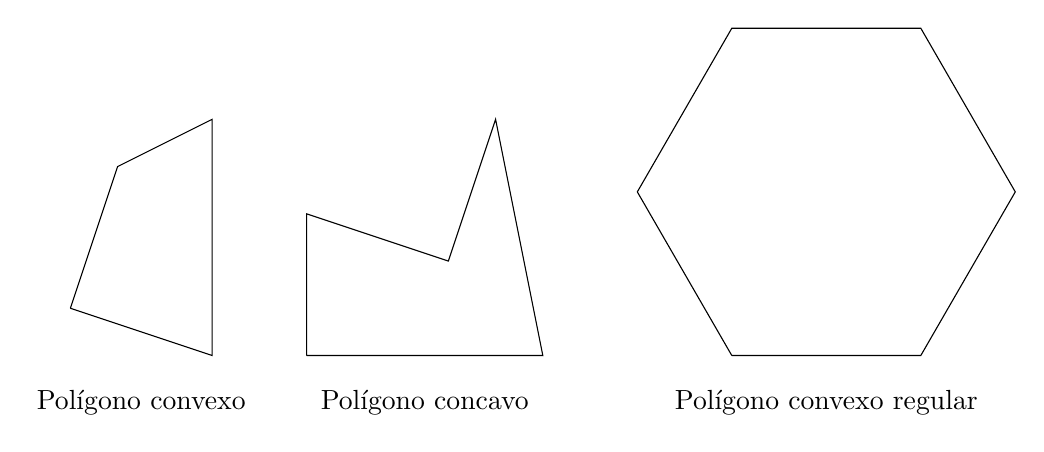
\begin{tikzpicture} [scale=0.6]
\draw (0,1) -- (3,0) -- (3,5) -- (1,4) -- (0,1);
\draw (5,0) -- (10,0) -- (9,5) -- (8,2) -- (5,3) -- (5,0);
\draw (14,0) -- (18,0) -- (20,3.464) -- (18,6.928) -- (14,6.928) -- (12,3.464) -- (14,0);
\node at (1.5,-1){Polígono convexo};
\node at (7.5,-1){Polígono concavo};
\node at (16,-1){Polígono convexo regular};
\end{tikzpicture}
\end{center}
\subsection{Triángulos}
- Los triángulos se pueden clasificar...
\begin{multicols}{2}
\begin{itemize}
\item \textbf{según sus lados:}
\begin{itemize}
\item Equilátero
\item Isósceles
\item Escaleno
\end{itemize}
\item \textbf{según sus ángulos:}
\begin{itemize}
\item Acutángulo
\item Rectángulo
\item Obtusángulo
\end{itemize}
\end{itemize}
\end{multicols}
\vspace{.5cm}
- Los elementos de un triángulo son:
\begin{itemize}
\item \textbf{Mediana}: es el segmento que une el punto medio de un lado con el vértice opuesto al mismo.
\item \textbf{Mediatriz}: es una recta perpendicular a un lado que pasa por su punto medio.
\item \textbf{Altura}: es el segmento perpendicular a un lado que pasa por su vértice opuesto.
\item \textbf{Bisectriz}: es la bisectriz de un ángulo.
\end{itemize}
\vspace{1cm}
- Y algunos puntos notables de un triángulo son:
\begin{itemize}
\item \textbf{Baricentro}: Las medianas se intersecan en un punto llamado baricentro, tal que su distancia a cada vértice es el doble a la distancia al punto medio del lado opuesto.
\item \textbf{Circuncentro}: Las mediatrices se intersecan en un punto llamado circuncentro, que es el centro de la circunferencia circunscripta al triángulo.
\item \textbf{Ortocentro}: Las rectas que contienen a las alturas se intersecan en un punto denominado ortocentro.
\item \textbf{Incentro}: Las bisectrices se intersecan en un punto denominado incentro, que es el centro de una circunferencia inscripta en el triángulo.
\end{itemize}
\subsection{Algunas Propiedades Importantes}
\begin{itemize}
\item En un $\triangle$ cada lado es menor que la suma de los otros dos, y mayor que su diferencia.
\item La suma de los ángulos interiores de un $\triangle$ es igual a un llano (180º).
\item El ángulo exterior a un $\triangle$ es igual a la suma de los dos interiores no adyacentes a él.
\item En un $\triangle$, a lados congruentes se oponen ángulos congruentes y viceversa.
\item En un $\triangle$, a mayor lado se opone mayor ángulo y viceversa.
\end{itemize}
\subsection{Congruencia de Triángulos}
Dos triángulos son \textbf{\textit{congruentes}} si tienen su lados y su ángulos respectivamente congruentes.\\ Dos triángulos son congruentes $\iff$
\begin{itemize}
\item Sus \textbf{tres lados} son respectivamente congruentes.
\item \textbf{Dos de sus lados y el ángulo comprendido} entre ellos son respectivamente congruentes. 
\item \textbf{Un lado y los ángulos con vértice en los extremos de dicho lado} son respectivamente congruentes.
\item \textbf{Dos de sus lados y el ángulo opuesto al mayor de los lados} son respectivamente congruentes.
\end{itemize}
\newpage
\subsection{Semejanza de Triángulos}
Dos $\triangle$ son \textbf{\textit{semejantes}} si tienen sus ángulos congruentes y sus lados homólogos proporcionales.\\
Dos triángulos son semejantes $\iff$
\begin{itemize}
\item Sus \textbf{tres lados} son proporcionales.
\item \textbf{Dos de sus lados} son proporcionales \textbf{y los ángulos comprendidos} entre ellos son congruentes.
\item \textbf{Tiene un par de ángulos} respectivamente congruentes.
\end{itemize}
\subsection{Polígonos (de más de tres lados)}
\textbf{Propiedades de polígonos convexos}:\\
La suma de los ángulos interiores de un polígono de $n$ lados se representa como:
\begin{center}
\framebox[8cm][c]{$S_n = (n-2) . 180$º}
\end{center}
Esto es porque la suma de los ángulos exteriores de un polígono de n lados es igual a 360º.
\subsection{Circunferencias}
Se define a una circunferencia como el lugar geométrico de los puntos del plano que equidistan de uno fijo, llamado centro. Las posiciones relativas de una recta y una circunferencia, y entre dos circunferencias, son:
\begin{itemize}
\item Una recta es \textbf{exterior} a una circunferencia si no tienen puntos en común.
\item Una recta es \textbf{tangente} a una circunferencia si tienen \textbf{solo} un punto en común.
\item Una recta es \textbf{secante} a una circunferencia si se intersecan en dos puntos.
\item Dos circunferencias son \textbf{secantes} si tienen dos puntos en común.
\item Dos circunferencias son \textbf{tangentes} si tienen solo un punto en común.
\item Dos circunferencias son \textbf{conceéntricas} si tienen el mismo centro.
\end{itemize}
\subsection{Elementos de una Circunferencia}
\begin{multicols}{2}
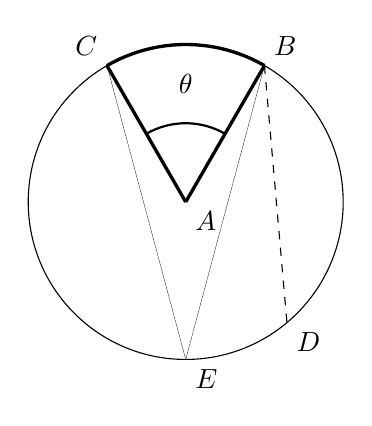
\begin{tikzpicture}[scale=2]
\coordinate [label=below right: $A$] (A) at (0,0);
\node[draw] (ci) at (A) [circle through=(right:1)] {};
\coordinate [label=above left:$C$] (C) at (ci.120);
\draw [very thick] (C) -- (A);
\coordinate [label=above right:$B$] (B) at (ci.60);
\draw [very thick] (B) -- (A);
\coordinate [label=below right:$ D$] (D) at (ci.310);
\draw [dashed] (B) -- (D);
\draw [black, very thick, domain=120:60] plot ({cos(\x)}, {sin(\x)});

\coordinate [label=below right:$E$] (E) at (ci.270);
\draw [ultra thin] (B)--(E);
\draw [ultra thin] (C)--(E);
\pic ["$\theta$", draw=black, thick, -, angle eccentricity=1.5, angle radius=1cm] {angle = B--A--C};
\end{tikzpicture}
\begin{itemize}
\item \textbf{BD Cuerda}, segmento cuyos extremos están en la circunferencia.
\item \textbf{CD Diámetro}, mayor de las cuerdas y contiene al centro de la circunferencia.
\item \textbf{AC Radio}, segmento cuyos extremos son el centro de la circunferencia y un punto de la misma.
\item \textbf{$\widearc{CB}$ arco}, subconjunto de la circunferencia.
\end{itemize}
\end{multicols}
\begin{itemize}
\item \textbf{$C\hat{A}B$ ángulo central} que se relaciona con el arco $\widearc{CB}$ es un ángulo cuyo vértice es el centro de la circunferencia y sus lados pasan por los extremos del arco al cual se lo relaciona.
\item \textbf{$C\hat{E}B$ ángulo inscripto} en la circunferencia que abarca el arco $\widearc{CB}$, es un ángulo cuyo vértice está en la circunferencia y sus lados pasan por los extremos del arco al cual se lo relaciona.
\end{itemize}
Propiedades:
\begin{itemize}
\item \framebox[2.5cm][c]{$C\hat{E}B = \dfrac{1}{2}C\hat{A}B$} Un ángulo inscripto es congruente con la mitad del central que abarca el mismo arco.
\item \framebox[2.5cm][c]{$C\hat{E}B = C\hat{D}B$} Los ángulos inscriptos en un mismo arco son congruentes.\\
\end{itemize}
\newpage
\subsection{Perímetros}
\end{document}